\section{System Architecture}\label{sec:system}

\begin{figure}[t]
\centering
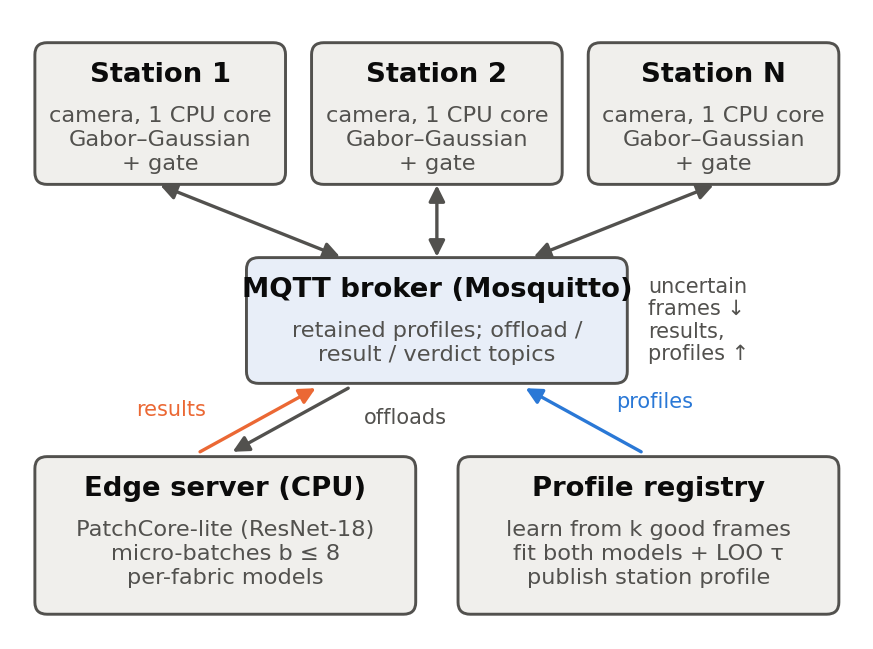
\includegraphics[width=\columnwidth]{fig_architecture.png}
\caption{FabricInspect-IoT. The registry learns a fabric once from $k$ defect-free frames, publishes the compact station model as a retained MQTT message, and installs the deep model on the edge. Stations score every frame and offload only uncertain ones.}
\label{fig:arch}
\end{figure}

Fig.~\ref{fig:arch} shows the three tiers. \emph{Station node:} each seaming machine carries a USB camera looking at the fabric in front of the seam line and a small computer (in our installation the machine's Android controller; in the experiments one CPU core). It holds only the station profile of the current fabric, scores each frame with the Gabor--Gaussian detector (Section~\ref{sec:gg}), and applies the confidence gate (Section~\ref{sec:gate}). \emph{Edge server:} one plant-level x86 machine without GPU subscribes to the offloaded frames of all stations, groups pending requests into micro-batches of up to $b_{\max}=8$, scores them with the PatchCore-lite model of the corresponding fabric (Section~\ref{sec:pc}), and returns the result. \emph{Profile registry:} when an operator learns a new fabric, the registry fits both models from the same $k$ frames, computes both thresholds, publishes the station profile as a \emph{retained} MQTT message, and stores the edge profile on the server. Because the broker keeps the last retained message per topic, a station that starts, reboots, or switches to that fabric receives the model immediately on subscription.

All communication uses MQTT~3.1.1~\cite{mqtt311} through a standard broker (Mosquitto~\cite{light2017mosquitto}) on four topics: \texttt{fi/profile/<fabric>/gabor} (station model, QoS~1, retained), \texttt{fi/st/<id>/offload} (JSON header plus $256\times256$ JPEG crop at quality 85, QoS~1), \texttt{fi/st/<id>/result} (JSON score and verdict, QoS~1), and \texttt{fi/st/<id>/verdict} (informational, QoS~0).

In \emph{learn} mode the operator slowly moves defect-free material under the camera while a frame is grabbed every 0.4\,s until $k$ frames (default 10) are collected. In \emph{inspect} mode each frame is centre-cropped, scored, and shown with a heat-map whose above-threshold regions are outlined; every decision is logged and defective frames are saved for review. A desktop GUI, a command-line interface, and the three IoT roles share one detector module, so the numbers in this paper are produced by the code an operator runs. The implementation uses Python, OpenCV, SciPy, Eclipse Paho, and PyTorch (CPU) with public ImageNet ResNet-18 weights~\cite{he2016resnet}.
